\chapter{Mikrofonverstärker}

\begin{figure}[H]
    \centering
    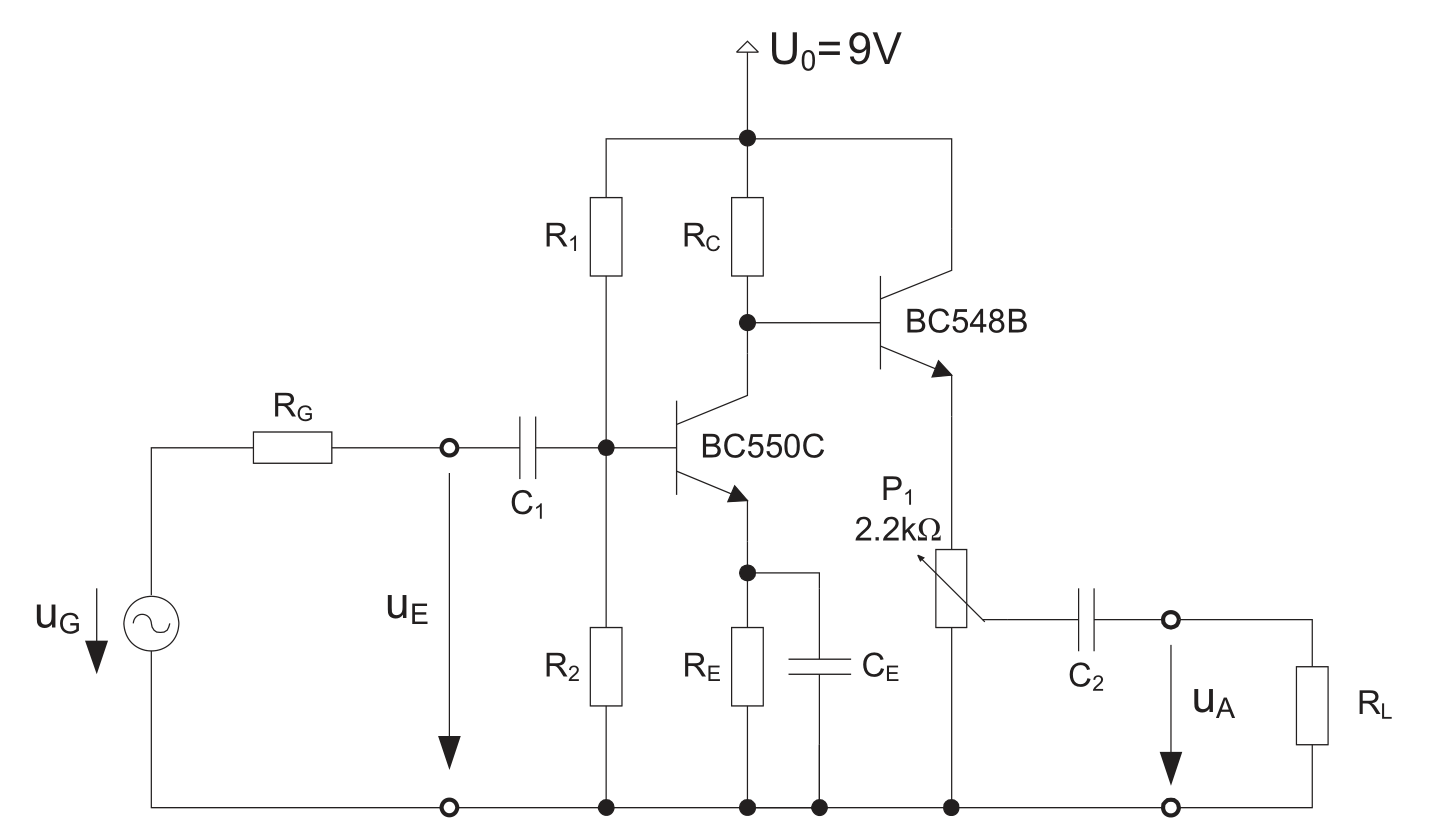
\includegraphics[width = \textwidth]{tex/1_Microphone/pictures/Schaltung.png}
    \caption{verwendete Schaltung}
\end{figure}

\section{Berechnung und Dimensionierun}
\subsection{Berechnung der Widerstände}
\subsubsection{Gegebene Randbedingungen}

\begin{itemize}
    \item Spannung an $R_E$: \SI{2}{\volt}
    \item Innenwiderstand der Signalquelle: \SI{4.7}{\kilo \ohm}
    \item Basisquerstrom $I_q$: \SI{0.1}{\milli \ampere} \ldots \SI{1}{\milli \ampere}
    \item Spannung am Emitter des zweiten Transistors: \SI{5}{\volt}
\end{itemize}

\subsubsection{Berechnung von $R_1$ und $R_2$}

Der Basisquerstrom wird durch die Widerstände $R_1$ und $R_2$ bestimmt (Der Basisstrom wird als vernachlässigbar klein gegenüber dem Querstrom angenommen).

\begin{equation*}
    I_q = \SI{0.5}{\milli \ampere} = \frac{U_0}{R_1 + R_2} \rightarrow R_1 + R_2 = \frac{U_0}{I_q} = \SI{18}{\kilo \ohm}
\end{equation*}

Weiters ist bekannt, dass an der Basis des BC550 etwa \SI{2.7}{\volt} anliegen (Emitterspannung + PN-Übergang). 

\begin{equation*}
    U_{B,0} = \SI{2.7}{\volt} = U_0 \frac{R_2}{R_1+R_2} \rightarrow \frac{R_2}{R_1+R_2} = \frac{U_{B,0}}{U_0} = \frac{2.7}{9} = 0.3
    \rightarrow R_1 = 2.3 \ R_2
\end{equation*}

In einer ersten Abschätzung ergeben sich somit folgende Werte für $R_1$ und $R_2$:

\begin{equation*}
    R_1 = \SI{12.545}{\kilo \ohm} \quad R_2 = \SI{5.454}{\kilo \ohm}
\end{equation*}

Gerundet auf die nähestenden Werte der E24-Reihe ergeben sich Widerstandswerte von:

\begin{equation*}
    R_1 = \SI{13}{\kilo \ohm} \quad R_2 = \SI{5.6}{\kilo \ohm}
\end{equation*}

Dies führt zu folgenden Schaltungsparametern:

\begin{equation*}
    I_q = \SI{484}{\milli \ampere} \quad U_{B,0} = \SI{2.710}{\volt}
\end{equation*}

In dieser Berechnung wurden einige Vereinfachungen durchgeführt, wie zutreffend dieses Ergebnis ist, muss durch die Simulation geprüft werden.

\subsubsection{Abschätzung des idealen Kollektorstroms}

Der optimale Kollektorstrom für einen möglichst rauscharmen Verstärker wird mit Gleichung 2.1 aus dem Praktikumsskript bestimmt:

\begin{equation*}
    R_0 = \sqrt{\frac{2 \ \beta \  r_{BB}}{I_{C0}}U_T + \frac{\beta}{ {I_{C0}}^2 }U_{T}^2}
\end{equation*}

umgeformt auf den gesuchten Strom ergibt sich:

\begin{align*}
    0 &= R_0^2 I_{C0}^2 - 2 \ \beta  r_{BB}  U_T  I_{C0} - \beta U_{T}^2 \\
    I_{C0} &= \frac{2 \ \beta  r_{BB}  U_T \pm \sqrt{\left( 2 \ \beta  r_{BB}  U_T\right)^2 + 4  R_{0}^2 \beta U_{T}^2 }}{2 R_{0}^2} \\
    I_{C0} &= U_T \frac{ \ \beta  r_{BB} \pm \sqrt{ \beta^2  r_{BB}^2 +  R_{0}^2 \beta }}{ R_{0}^2} \\
    I_{C0} &= \SI{25}{\milli \volt} \frac{600 \cdot \SI{150}{\ohm} \pm \sqrt{(600 \cdot \SI{150}{\ohm})^2 + (\SI{2136}{\ohm})^2 \cdot 600}}{(\SI{2136}{\ohm})^2} = \SI{1.064}{\milli \ampere}, \SI{-77.28}{\micro \ampere}
\end{align*}

Das negative Ergebnis für $I_{C0}$ wird als nicht-physikalisch interpretiert und verworfen, weitergerechnet wird mit $I_{C0} = \SI{1}{\milli \ampere}$

Verwendeete Werte:

\begin{itemize}
    \item Kleinsignalverstärkung des BC550C \emph{typ.: }$\beta = 600$
    \item Basisbahnwiderstand \emph{Base Spreading Resistance}: $r_{BB} \approx \SI{150}{\ohm}$ \\
    Anm.: $r_{BB}$ ist eine funktion von $I_{C0}$, dieser Wert gilt für ca. \SI{3}{\milli\ampere}, bei großer Abweichung muss iterativ eingesetzt werden.
    \item Temperaturspannung: $U_T = \frac{k_b T}{e} = \SI{25}{\milli \volt}$ \\
    Anm.: Dieser Wert gilt bei Raumtemperatur, je nach Temperatur bzw. Verlustleistung des Transistors ist dieser Wert zu hinterfragen.
    \item Generatorwiderstand $R_0 = \left( G_1 + G_2 + G_G\right)^{-1} = \SI{2136}{\ohm}$
\end{itemize}

\subsubsection{Berechnung von $R_E$ und $R_C$}

Durch $R_E$ und $R_C$ fließen im wesentlichen der eben berechnete Kollektorstrom (der Basisstrom wird vernachlässigt).

\begin{equation*}
    U_{R_{E}} = \SI{2}{\volt} = I_{C0} R_E \rightarrow R_E = \SI{2}{\kilo \ohm}
\end{equation*}

Der Kollektor des ersten Transistors ist an der Basis des zweiten Transistors angeschlossen. Dessen Emitter soll auf einem Potential von etwa \SI{5}{\volt} liegen. Damit liegt die Basis dieses zweiten Transistors auf \SI{5.7}{\volt}.

\begin{equation*}
    \SI{9}{\volt} - \SI{5.7}{\volt} = I_{C0} R_C \rightarrow R_C = \SI{3.3}{\kilo \ohm}
\end{equation*}

\subsection{Abschätzung von Ein- und Ausgangswiderstand}
\subsection{Bode-Plot}
\subsubsection{Simulieren Sie mit einer geeigneten Analyseart und Beschaltung den Amplituden- und Phasengang des Operationsverstärkers.}

Für diese Fragestellung eignet sich die AC-Sweep-Simulation. Hierfür wird die $V_{IN}$ zu einer Wechselspannungsquelle mit Spannungsamplitude \SI{1}{\volt} konfiguriert. In der AC-Simulation wird um den Arbeitspunkt linearisiert, eventuelle Austeuergrenzen und Sättigung spielen bei dieser Simulation keine Rolle. Simuliert wurde ein Frequenzbereich von \SI{1}{Hz} bis \SI{10}{\mega \hertz}.

\begin{figure}[H]
    \centering
    \includegraphics[width = \textwidth]{Bilder/Schaltung_2.png}
    \caption{verwendete Schaltung und Simulationsparameter}
    \label{fig:my_label}
\end{figure}

\textbf{Simulationsergebnis:} Das resultierende Bode-Diagram:
\begin{figure}[H]
    \centering
    \includegraphics[width = \textwidth]{Bilder/BodePlot.pdf}
    \caption{Frequenzgang}
    \label{fig:my_label}
\end{figure}

\subsubsection{Welche Verstärkung $A_0$ besitzt der Verstärker?}

Der Operationsverstärker besitzt eine Open-Loop-Verstärkung $A_0 = \frac{U_{OUT}}{U_{INP}-U_{INN}}$ von \num{3.74e4} beziehungsweise \SI{91.4}{dB}.

\subsubsection{Beeinflusst die Offsetspannung den Frequenzgang?}

Nein, die Offsetspannung hat keinen Einfluss auf den Frequenzgang, da die Schaltung für die Berechnung des Frequenzganges um den Arbeitspunkt linearisiert wird, es wird quasi mit dem Kleinsignalersatzschaltbild gerechnet.

\subsubsection{Welches GBW besitzt der OPV?}

Der Amplitudengang durchschreitet die \SI{0}{dB}-Linie bei einer Frequenz von \SI{1.13}{\mega \hertz}, dies entspricht auch dem Gain-Bandwith-Product.

\subsubsection{Wie kann die Verstärkung $A_0$ des OPV verändert werden?}

Die Open-Loop-Verstärkung $A_0$ ist eine Eigenschaft des OPVs und kann nicht durch externe Beschaltung verändert werden. Diese Verstärkung wird im wesentlichen durch die Spannungs-Verstärkungs-Stufe des OPVs bestimmt.

\subsection{Slew-Rate}

\subsubsection{Bestimmen Sie die Slew-Rate des OPV mit geeigneter Beschaltung.}

Zur Bestimmung der Slew-Rate wird der OPV als Impedanzwandler oder Spannungsfolger verschaltet, der Ausgang wird also auf den invertierenden Eingang rückgeführt. Als Eingangssignal wird eine Folge von Rechteckimpulsen aufgeschalten. Die Slew-Rate ist dann die Geschwindigkeit in der das Ausgangssignal diesem Impuls folgt.

\begin{figure}[H]
    \centering
    \includegraphics[width = \textwidth]{Bilder/Schaltung_3.png}
    \caption{Bufferschaltung zur Bestimmung der Slew-Rate}
    \label{fig:my_label}
\end{figure}

\textbf{Simulationsergebnis:} Es ergab sich folgender zeitlicher Verlauf der Ausgangsspannung und folgende Werte für die Slew-rate:

\begin{table}[H]
    \centering
    \begin{tabular}{|c|c|}
    \hline
         steigende Flanke & fallende Flanke  \\ \hline
         \SI{741}{\kilo \volt \per \second} & \SI{-5.11}{\mega \volt \per \second} \\ \hline
    \end{tabular}
    \caption{Caption}
    \label{tab:my_label}
\end{table}
\begin{figure}[H]
    \centering
    \includegraphics[width = \textwidth]{Bilder/Slewrate_default.pdf}
    \caption{Zeitlicher Verlauf der Spannungen}
\end{figure}

\subsubsection{Warum unterscheidet sich die Slew-Rate für die fallende und steigende Flanke}

Die Ursache für den Unterschied zwischen der Slew-Rate bei steigender und fallender Flanke ist vermutlich in der Ausgangsstufe des OPVs zu suchen. Bei steigender Flanke muss die Kapazität erst geladen werden, dies erfordert kurzzeitig hohe Ströme und hohe Leistungen. $\rightarrow$ Bei der steigenden Flanke ist man durch den maximalen Ausgangsstrom des OPV limitiert, bei der fallenden Flanke hingegen ist der maximale Sink-Current entscheidend, der typischerweise um einiges größer ist.

\subsubsection{Hat die Last einen Einfluss auf die Slew-Rate?}

Die Last hat einen sehr großen Einfluss auf die Slew-Rate. Ein größerer Kondensator würde z.B. mehr Ladung brauchen um auf die selbe Spannung geladen zu werden, um dies in der gleichen Zeit zu schaffen also mehr Leistung.\\

\textbf{Simulation mit der Last $C_1 = \SI{1}{\nano \farad}, R_3 = \SI{10}{\mega \ohm}$:}

\begin{table}[H]
    \centering
    \begin{tabular}{|c|c|}
    \hline
         steigende Flanke & fallende Flanke  \\ \hline
         \SI{33.3}{\kilo \volt \per \second} & \SI{-961}{\kilo \volt \per \second} \\ \hline
    \end{tabular}
    \caption{Caption}
    \label{tab:my_label}
\end{table}

\begin{figure}[H]
    \centering
    \includegraphics[width = \textwidth]{Bilder/Slewrate_1n.pdf}
    \caption{Zeitlicher Verlauf der Spannungen mit veränderter Last}
\end{figure}

Bei kleinerer Last lässt sich hingegen eine schnellere Slew-Rate beobachten. Auffällig ist auch, dass sich die Geschwindigkeiten für steigende und fallende Flanken annähern:

\textbf{Simulation mit der Last $C_1 = \SI{1}{\pico \farad}, R_3 = \SI{20}{\mega \ohm}$:}

\begin{table}[H]
    \centering
    \begin{tabular}{|c|c|}
    \hline
         steigende Flanke & fallende Flanke  \\ \hline
         \SI{5.55}{\mega \volt \per \second} & \SI{-5.47}{\mega \volt \per \second} \\ \hline
    \end{tabular}
    \caption{Caption}
    \label{tab:my_label}
\end{table}

\begin{figure}[H]
    \centering
    \includegraphics[width = \textwidth]{Bilder/Slewrate_1p.pdf}
    \caption{Zeitlicher Verlauf der Spannungen mit veränderter Last}
\end{figure}

\section{Simulation in LTSpcie}

\section{Anhang:}

Die Simulationen wurden mit LTSpice XVII durchgeführt. Die Diagramme wurden durch Datenexport von LTSpice mit Matplotlib erstellt.